\section{Lack of Annotated Datasets}
\label{sec:introduction:lack_of_annotated_datasets}

A primary challenge in performing a systematic analysis of the discursive functions of LoL esports shoutcasting is the lack of annotated datasets of shoutcasting transcripts. 

\medskip

In the domain of esports and audience engagement, previous studies have been focused on building different kinds of collaborative shoutcasting \cite{huang2022sentence}. Additionally, most statistical analyses have been done with the purpose of creating XAI and visualization tools with existing game-data \cite{pedrassoli2024exploration, kokkinakis2020dax}. These studies will be covered in greater detail in the next chapter. While they provide valuable insights on audience engagement, they do not address the linguistic and discursive properties of commentary but instead focus on more structured and easily processed in-game data.

\medskip

To our knowledge, existing studies that analyze commentary content are limited, focusing on a single discourse type, namely storytelling, and only in the domain of traditional sports \cite{lee2014automated}.

\medskip

This represents a core obstacle for an Artificial Intelligence approach to the analysis of discursive functions, since models for discourse studies have required substantial amounts of data just for evaluation and benchmarking \cite{qingyu2025deploying}.

\medskip

To address this limitation, this research proposes the development of an annotation framework for esports commentary, taking advantage of the existing availability of professional game recordings and corresponding Video-on-Demand (VOD) which include shoutcaster transcripts. 

\medskip

\begin{figure}
  \centering
  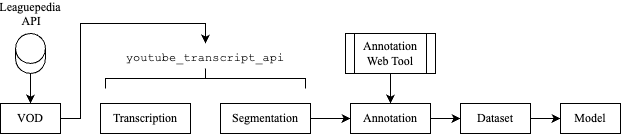
\includegraphics[width=\textwidth]{chapters/01_introduction/images/thesis-workflow.png}
  \caption{Proposed annotation pipeline for League of Legends esports shoutcasting data, from raw VOD recordings to labeled discourse data for computational analysis.}
  \label{fig:annotation_pipeline}
\end{figure}

To facilitate the data collection process, we are developing a web-based annotation tool, which will divide the VOD transcriptions into labelleable segments. The goal of this tool is to improve annotation efficiency and enable Human-in-the-Loop (HITL) workflow in the future as a part of this research, as observed in Figure \ref{fig:annotation_pipeline}. 

\medskip

Early experiments with this tool will also allow us to form preliminary research questions, and identify relevant discursive functions for analysis. This will ensure that the framework and modeling is grounded in empirical observations. 